




% Template for PLoS
% Version 1.0 January 2009
%
% To compile to pdf, run:
% latex plos.template
% bibtex plos.template
% latex plos.template
% latex plos.template
% dvipdf plos.template

\documentclass[10pt]{article}

% amsmath package, useful for mathematical formulas
\usepackage{amsmath}
% amssymb package, useful for mathematical symbols
\usepackage{amssymb}

% graphicx package, useful for including eps and pdf graphics
% include graphics with the command \inputgraphics
\usepackage{graphicx}
\usepackage{lscape}

% cite package, to clean up citations in the main text. Do not remove.
\usepackage{cite}

\usepackage{color} 

% Use doublespacing - comment out for single spacing
\usepackage{setspace} 
\doublespacing


% Text layout
\topmargin 0cm
\oddsidemargin 0.5cm
\evensidemargin 0.5cm
\textwidth 16cm 
\textheight 21cm

% Bold the 'Figure #' in the caption and separate it with a period
% Captions will be left justified
\usepackage[labelfont=bf,labelsep=period,justification=raggedright]{caption}

%load my own packages (not PLoS template)
\usepackage{textcomp, fixltx2e}
\usepackage{fullpage, lscape}
\usepackage{lineno}

% Use the PLoS provided bibtex style
\bibliographystyle{plos2009}

% Remove brackets from numbering in List of References
\makeatletter
\renewcommand{\@biblabel}[1]{\quad#1.}
\makeatother


% Leave date blank
\date{}

\pagestyle{myheadings}
%% ** EDIT HERE **


%% ** EDIT HERE **
%% PLEASE INCLUDE ALL MACROS BELOW

%% END MACROS SECTION

\usepackage{Sweave}
\begin{document}

% Title must be 150 characters or less
\begin{flushleft}
{\Large
\textbf{Controls of litter chemistry over early lignin decomposition in beech litter}
}
\\
% Insert Author names, affiliations and corresponding author email.
% Insert Author names, affiliations and corresponding author email.
Lukas Kohl$^{1}$, % $^{3,\ast}$
Wolfgang Wanek$^{1}$, 
Katharina Keiblinger$^{2,3}$, 
Sonja Leitner$^{1,3}$, 
Maria Mooshammer$^{1}$, 
Ieda H\"ammerle$^{1}$, 
Lucia Fuchslueger$^{1}$, 
J\"org Schnecker$^{1}$, 
Thomas Schneider$^{4,5}$
Sandra Moll$^{7}$
Markus Gorfer$^{7,8}$
Joseph Strauss$^{7,8}$
Katharina Riedel$^{4,6}$
Leo Eberl$^{4,5}$
Sophie Zechmeister-Boltenstern$^{2,3}$, 
Andreas Richter$^{1}$,
\\
\bf{1} Department of Chemical Ecology and Ecosystem Research, University of Vienna, Althanstrasse 14, A-1090 Vienna, Austria
\\
\bf{2} Federal Research and Training Centre for Forests, Natural Hazards and Landscape, Department of Soil Biology, Seckendorff-Gudent-Weg 8, A-1131 Vienna, Austria
\\
\bf{3} Current address: Institute for Soil Science, University of Natural Resources and Life Sciences, Peter Jordan-Stra\ss e 82, A-1180, Vienna, Austria
\\
\bf{4} Institute of Plant Biology, University of Zurich, Winterthurerstrasse 190, CH-8057, Zurich, Switzerland
\\
\bf{5} Current address: Institute of Plant Biology, University of Zurich, Zollikerstrasse 107, CH-8008, Zurich, Switzerland
\\
\bf{6} Current address: Institute of Microbiology, Ernst-Moritz-Arndt University of Greifswald, Friedrich-Ludwig-Jahn-Strasse 15, D-17487 Greifswald, Germany
\\
\bf{7} Fungal Genetics and Genomics Unit, Department of Applied Genetics and Cell Biology, University of Natural Resources and Life Sciences, Konrad-Lorenz-Strasse 24, A-3430 Tulln, Austria
\\
\bf{8} AIT Austrian Institute of Technology GmbH, Bioresources Unit, Konrad-Lorenz-Strasse 24, A-3430 Tulln, Austria

$\ast$ E-mail: Corresponding author@institute.edu
\end{flushleft}

\newpage
% Please keep the abstract between 250 and 300 words
\section*{Abstract}

Lignin is a major component of plant litter and is considered highly resistant to decomposition. Carbohydrates, in contrast, are more easily degraded. We studied the decomposition rates of these two compound classes, and to which extent they are controlled by litter C:N:P stoichiometry. 

Herein we report results from a 15-months mesocosm experiment under controlled climatic conditions with beech litter of different N and P contents. Litter was sterilized and re-inoculated prior to the experiment to minimize differences in the initial microbial community, but study the effect of N and P contents on identical initial decomposer communities. Lignin and carbohydrate decomposition rates were determined by pyrolysis-GC/MS for 2 periods (0-6 months and 6-15 months), the composition of the microbial community was monitored via metaproteome analysis.

Different in litter nutrient contents led to the establishment of different decomposer communities. Fungi were dominant on all litter, but fungi:bacteria ratios were highest on high-nutrient litter, leading to a negative correlation between litter and microbial stoichiometry and high differences between litter and microbial C:N and C:P ratios on nutrient poor litter.

Rates of lignin decomposition were highly variable during the first six months, ranging from insignificant amounts decomposed to decomposition at bulk C mineralization rates. Between 6 and 15 months, lignin was degraded at bulk mass loss rates independent of the litter nutrient contents, however, different lignin contents aquired within the initial 6 months remained in place. Early lignin degradation rates were highest in litter with low fungi:bacteria ratios, and were correlated to differences between litter and microbial stoichiometry (C:P$_{litter : microbial}$ and C:P$_{litter : microbial}$). Lignin degrading communities were enriched in $\gamma$-proteobacteria after 6 months incubation.

Our results indicate that - contradicting common models - significant amounts of lignin were be degraded during early decomposition in low nutrient litter. We demonstrate that litter quality profoundly affects the lignin decomposition via the composition of the decomposer community. Even though bacterial biomass is enriched in N and P, communities low nutrient litter were enriched in bacteria. This led to higher differences between litter and microbial stoichiomety, a possible control over lignin degradation during early decomposition. 

\linenumbers %not from the template: start line numbers here.
\newpage%not in original layout
\input{introduction}
% Results and Discussion can be combined.
\section*{Results}
\subsection*{Initial litter chemistry}
Initial litter chemistry of the four sites (Achenkirch, AK, Klausenleopoldsdorf, KL, Ossiach, OS, Schottenwald, SW), measured 14 days after incubation, is presented in supplemental table \ref{initstoech}. C:N ratios varied between 41:1 and 58:1 and C:P ratios between 700:1 and 1300:1, while N:P ratios ranged between 15:1 and 30:1. No significant changes occurred during litter incubation except a slight decrease of the C:N ratio (41.8:1 to 37.4:1) found in the most active litter type (SW) after 15 months. Fe concentrations were more than twice as high for OS (approx. 450 ppm) than for other litter types (approx. 200 ppm). Litter Mn also was highly variable between litter types, ranging between 170 and 2130 ppm. Changes of micro-nutrient concentrations during litter incubation were significant, but in all cases \textless 15\% of the initial concentration. In initial litter, lignin accounted for 28.9-31.2\% and carbohydrates for 25.9-29.2\% of the total peak area of all pyrolysis products.

\subsection*{Mass loss, respiration and soluble organic carbon}

Litter mass loss was not significant after 2 weeks and 3 months, and significant for 2 litter from two sites after 6 months. After 15 months, litter mass loss was significant for all collection sites, and ranged between 5 and 12 \% of the initial dry mass, and was strongly correlated to litter N content (R=0.794, p\textless 0.001). Detailed results were reported by \cite{Mooshammer2011}.

Highest respiration rates were measured at the first measurement after 14 days incubation (150-350 \textmu g CO$_2$-C d$^{-1}$ g$^{-1}$ litter-C), which dropped to 75 to 100 \textmu g CO$_2$-C d$^{-1}$ g$^{-1}$ litter-C after 3 months. After 6 and 15 months, respiration rates for AK and OS further decreased, while SW and KL showed a second maximum in respiration after 6 months (fig \ref{fig:enz}). Accumulated respiration was strongly correlated to litter mass loss after 15 months (r=0.738, p\textless 0.001, n=20).

Soluble organic carbon concentrations decreased between the first three harvests (14 days to 6 months), and strongly increased to 15 months (from 0.1 to 0.7 mg C g$^{-1}$  d.w. to 1.5 to 4 mg C g$^{-1}$ d.w. after 15 months, fig. \ref{fig:enz}). After 14 days and 3 months, the highest soluble organic C concentrations were found in SW litter followed by AK. Soluble organic C concentrations were weakly correlated with litter N content after 14 days (r=0.69, p\textless 0.001, n=20) and after 3 months (r = 0.65, p\textless 0.01, n=20), but strictly correlated after 6 months (r=0.85, p\textless 0.001, n=20) and 15 months (r=0.90, p\textless 0.001, n=20).

\subsubsection*{Potential enzyme activities}
Within each time point, all potential extracellular enzyme activities were correlated with litter N and actual respiration rates(all R\textgreater 0.8, p\textless 0.001, n=20). Cellulase activity increased from the first harvest onwards to 15 months, with a small depression after 6 months (Fig. \ref{fig:enz}), phenoloxidase and peroxidase activities reached their maximum between 3 and 6 months (fig. \ref{fig:enz}). For all enzymes and at all time points, SW showed the highest and AK the lowest activities. Differences between these two sites were more pronounced in cellulase activity (SW 10x higher than AK) than in oxidative enzymes (SW 4x higher). Conversely, the phenoloxidase/cellulase ratio was highest for AK and lowest for SW at all time points and decreased during litter decomposition (fig. \ref{fig:enz}).

\subsubsection*{Microbial biomass abundance and community composition}
Microbial biomass contents ranged from 0.5 to 6 mg C g$^{-1}$ d.w., 0.05 to 0.55 mg N g$^{-1}$ d.w. and 0.05 to 0.35 mg P g$^{-1}$ litter d.w (fig. \ref{fig:mb}). After an initial increase in microbial biomass, in KL and OS microbial biomass remained constant after 3 months while AK and SW showed further microbial biomass growth reaching a maximum of microbial C and N contents after 6 months (AK also for P). Microbial C:N ratios ranged between 6:1 and 18:1, C:P ratios between 8:1 and 35:1, and N:P ratios between 0.5:1 and 3.5:1 (fig. \ref{fig:mb}).

Microbial biomass was stoichiometrically homeostatic during the first 6 months (no or negative correlations between microbial C:N:P and litter C:N:P, see also \cite{Mooshammer2011}), but after 15 months (microbial C:N:P ratios were significantly and positively correlated to resource stoichiometry: R=0.53-0.64, all p\textless 0.002). The homeostatic regulation coefficients \cite{Sterner2002} were H\textsubscript{C:P}=1.68, H\textsubscript{C:N}=2.01, and H\textsubscript{N:P}=2.29 after 15 month incubation. Microbial C:N ratios after 3 and 6 months were within a tighly constrained range, 14.5:1 to 18.2:1 after 3 months and 6.9:1 to 9.0:1 after 6 months, but significantly different between the two sampling events. In contrast, microbial C:P and N:P ratios were less constrained, with the highest variance between litter from different sites after 3 months of incubation (fig. \ref{fig:mb}).

Metaproteome analysis yielded between 451 and 1113 (average 639) assigned spectra sample (one replicate per collection site after 14 days, 3, 6, and 15 months). Only spectra assigned to bacteria or fungi were used for community profiling. Fungal proteins were dominant in all litter types at all stages, but most prominent in SW and least pronounced in  AK. Fungi:bacteria (F:B) protein abundance ratios were highest after 14 days (5 to 12) and decreased during litter decomposition (1.7 to 3 after 15 months, see fig. \ref{fig:f2b}). The large initial differences in F:B ratios between litter from different sites decreased during decomposition. In addition, F:B ratios were measured on a DNA basis (qPCR) the results showing a similar pattern but with a much larger fungal DNA dominance (F:B ratios between 10-180). F:B ratios were highly correlated between protein- and log-transformed DNA-based estimates (r=0.785, p\textless 0.001, n=20).

Fungal communities were dominated by Ascomycetes, with smaller contributions by Basidiomycetes (<5\% of fungal protein).  Among the fungal classes found, Sordariomycetes and Eurotiomycetes were most abundant with further contributions of Dothideomycetes, Leothiomycetes and Saccharomycetes (fig. \ref{fig:metaprot_barplot}). Bacteria were dominated by Proteobacteria (mainly $\gamma$, declining, and $\alpha$- and $\beta$-Proteobacteria, increasing with litter decomposition) with minor contribution of Actinomycetes and Bacterioidetes (both increasing) and Thermotogae (decreasing, fig. \ref{fig:metaprot_barplot}).

\subsection*{Pyrolysis-GC/MS and Lignin content}
In total 128 pyrolysis products were detected, quantified, identified and assigned to their substances of origin (suppl. tab. \ref{tab:phprod} -\ref{tab:nprod}). We found only minor changes in the relative concentration of litter pyrolysis products during decomposition, and differences between sites were small but well preserved during decomposition. However, the high precision and reproducibility of pyrolysis GC/MS analysis of litter allowed tracing small changes in lignin and carbohydrate abundance during decomposition. Lignin-derived compounds made up between 29 and 31 \% relative peak area (TIC) in initial litter, and increased by up to 3 \%. The increase occured almost exclusively during the first 6 months. Carbohydrate-derived pyrolysis products accounted for 26 to 29 \% in initial litter and decreased by up to 2.6 \% within 15 months of incubation. The initial (pyrolysis-based) lignin:carbohydrate indices (LCI) were highly similar between litter from different collection sites, ranging between 0.517 and 0.533 (Fig. 4). During decomposition, the LCI increased by up to 9 \% of the initial value. The highest increase was found in SW litter, while LCI slightly decreased in AK litter. All significant changes in LCI  occurred within the first 6 months (fig. \ref{fig:lci}). As differences in lignin and carbohydrate contents between 0-3 and 3-6 months were not significant, we analyzed differences for two time intervals, i.e. between 0-6 months and 6-15 months.

During the first 6 months, between one and 6 \% of the initial lignin pool and between 4 and 17\% of the initial carbohydrate pool were degraded (Fig. \ref{fig:degr}). Lignin decomposition was highest in AK and KL litter, while microbial communities of KL, OS and SW litter decomposed carbohydrates faster. Lignin preference values (\% lignin decomposed : \%carbohydrates decomposed) were lowest in SW and highest in AK litter (Figure 5). In AK litter, lignin macromolecules were 50 \% more likely to be decomposed than carbohydrates, while in SW litter carbohydrates were 10 times more likely to be decomposed (fig. \ref{fig:degr}). Between 6 and 15 months, no further accumulation of lignin occurred. Lignin and carbohydrates were both degraded at the same rate and their relative concentrations remained constant between 6 and 15 months (fig. \ref{fig:degr}).

\subsection*{Correlations between lignin and carbohydrate decomposition and litter chemistry, microbial community and decomposition processes}

Relationships between lignin and carbohydrate degradation, litter chemistry, microbial biomass and decomposition processes were tested after 6 and 15 months (tables \ref{corrtable} and \ref{corrtable2}) including data presented by \cite{Mooshammer2011} and \cite{Leitner2011}. After 6 months, we found that the ratio of lignin/cellulose degradation was positively correlated with the ratio of phenoloxidase : cellulase (R=0.599, p=0.005, n=20) and peroxidase : cellulase (R=0.734 p\textless 0.001, n=20). Carbohydrate decomposition was positively correlated with litter N content, and negatively with litter C:N ratios and litter-microbial C:N imbalances. In contrast, lignin decomposition was negatively correlated to litter P, but positively with litter C:P and N:P ratios, and litter-microbial C:P and N:P imbalances (fig. \ref{fig:cor1}). After 15 months, the ratio of lignin : carbohydrate decomposition was no longer related to stoichiometry or elemental composition any more. Most interestingly, lignin and carbohydrate decomposition exhibited the same controls, being positively correlated to soluble organic C, litter N and litter P (table \ref{corrtable2}) between 6 and 15 months. Mass loss and accumulated respiration were positively correlated to lignin and carbohydrate decomposition (table \ref{corrtable2}), a pattern that we did not find for lignin decomposition in the early decomposition phase (table \ref{corrtable}). Protein abundance F:B ratios were negatively correlated to the ratios of lignin : cellulose decomposition and to LCI change during the first 6 months, pointing to bacterial engagement in lignin decomposition. In contrast, both lignin and carbohydrate decomposition rates, were positively correlated with F:B ratios after 15 months, pointing to fungal dominance of both lignin and carbohydrate decompostion. No correlation between F:B ratio and the ratio of lignin : cellulose decomposition was found in this later period (fig. \ref{fig:f2b}).


To asses the interaction between litter chemistry, microbial community and degradation processes, we conducted a correspondence analysis (CA) of the metaprotomen data (relative protein abundances, fig. \ref{fig:metaprotpca}). The results indicate that incubations time (i.e. succession) is the dominant factor controlling the microbial community, with samples collected at the first (14 days) and the last (15 month) sampling grouping closely together, while litter quality (i.e. elemental stoichiometry of litter collected at different sites) had a higher impact after 3 and 6 months. The first factor (CA 1), which explained 35.7 \% of the total variance, separates litter sampled after 15 months (positive values) from litter sampled earlier (negative values). Consequently, CA 1 was also positively correlated to incubation time and negatively to litter carbon content (i.e. decreasing C:N ratios during decomposition) . A number of bacterial taxa (Actinobacteria, Bacteroidetes, Alpha- and Betaproteobacteria), and two fungal classes (Leotiomycetes and Tremellomycetes) were positively correlated to CA1 i.e. increased in abundance towards 15 months, while Cyanobacteria, Epsilonproteobacteria and Saccharomycetes were negatively correlated. CA 2, which explained 26.0 \% variance, separated litter sampled within the first 6 months. Dothideomycetes and Sordariomycetes were positively and Gammaproteobacteria negatively correlated to this factor, which also correlated to the F:B protein abundance ratio. Litter collected 14 days after inoculation have the highest scores on CA 2, while sites with active lignin degradation within the first 6 months (AK, KL) have the most negative scores. The axis was furthermore correlated to the microbial biomass P content and C:P and N:P imbalances (and free NH\textsubscript{4}\textsuperscript{+}, not shown). For samples analyzed after 6 months, where direct comparison to lignin degradation rates was possible, significant correlations to CA 2 were found for lignin : carbohydrate degradation (r=-0.97, p=0.028), \% Lignin loss : \% Carbon loss (r=-0.96, p=0.040) and  LCI increase (r=0.973, p=0.027), even though the number of independent samples was very low (n=4). Differences in CA2 strongly decreased after 15 months, suggesting that the differences in the microbial community found within the first 6 months were siminished with succession of the decomposer community. Litter N and P contents were not correlated to either factor, although differences in resource quality evidently affected community composition after 3 and 6 months, as can be seen in the differences in the microbial communities as observed in CA 2. Correlation of CA factors with litter stoichiometry, and microbial stoichiometry, and the abundance of the analyzed taxa are provided in supplemental table \ref{catab}.
\section*{Discussion}

The experimental approach chosen allowed us to single out the effects of litter quality on the microbial decomposer community and decomposition processes, while excluding effects of fauna, climate and different initial microbial communities. By exploiting intra-specific differences in beech litter stoichiometry, we were able to minimize differences in the chemical composition of initial litter (e.g. similar lignin and cellulose content, table \ref{initstoech}), while exploring the effect of litter nutrient contents on lignin and carbohydrate decomposition. Therefore, we can attribute different rates of carbohydrate and lignin decomposition to the intrinsic qualities of litter collected at different sites, i.e. elemental and stoichiometric composition. Analytical pyrolysis allowed specific determination of litter lignin contents (simultaneously with carbohydrates), avoiding the limitations of common methods for lignin quantification as AUR \cite{Hatfield2005}.

Contradicting traditional concepts of litter decomposition, our results demonstrate that variable amounts of lignin were degraded during the first 6 months of incubation. During this early stage, lignin decomposition rates depended on litter quality (P) and ranged from non-significant to degradation rates similar to bulk carbon mineralization rates (i.e. no discrimination against lignin). We can therefore confirm that early lignin decomposition rates are by far underestimated, as recently proposed by \cite{Klotzbucher2011}, based on a complementary analytic approach. Unlike \cite{Klotzbucher2011}, we found no decrease but constant or increasing lignin decomposition rates during litter decomposition over 15 months. 

Our results provide strong evidence that litter C:N:P stoichiometry and litter element concentrations exerted a major control on the extent of lignin decomposition during the initial decomposition phase. Carbohydrate decomposition was positively correlated with litter N contents and negatively to litter C:N ratios, as were the majority of decomposition processes (mass loss, respiration, potential extracellular enzymatic activities). In contrast, lignin decomposition rates were positively correlated with litter C:P ratios and negatively with dissolved and total litter P. The relationship was strongest when lignin decomposition rates were compared to litter-microbe C:P imbalances, i.e. the greater the imbalance between resource and consumer C:P became (greater P limitation) the lower lignin decomposition rates became. Additionally, we found a marked change in the controls of lignin decomposition during this period. While carbohydrate and lignin decomposition were differently controlled by litter chemistry (N versus P) during the first 6 months, these litter components were decomposed at similar rates thereafter and decomposition rates were only related to litter N availability. 

Cultivation studies showed that lignin decomposition by fungi is triggered by nitrogen starvation, and that lignin does not provide sufficient energy to maintain the decomposer's metabolism without the use of other organic C i.e. energy sources \cite{Janshekar1988}. Moreover, lignin decomposition was found in wild-type \emph{A. thaliana} litter containing abundant cellulose as a C source, but not in a low-cellulose mutant during a 12-month incubation experiment in a boreal forest \cite{Talbot2011}. In the N- and P-(co-)limited situation commonly encountered during early litter decomposition, we may speculate that lignin is degraded to access additional nutrients (mainly N) or to use a C surplus by decomposing a less C efficient but nutrient enriched substrate (nutrient mining hypothesis). However, a stimulation of lignin decomposition by low P availability or microbial P limitation, as indicated by the strong negative correlations to P pools that we found, has not been reported yet. Though lignified materials have been reported to be N-rich and decomposition of these materials may therefore enhance N supply to microbial communities, lignins are not expected to contain quantitative important amounts of P.

In order to decompose litter lignin and carbohydrates, microbial decomposers rely on the production and excretion of hydrolytic and oxidative extracellular enzymes. While the absolute amounts, in which these enzymes are produced, were largely controlled by N availability, the ratio in which they were produced was strongly related to differences in the ratio of cellulose:lignin decomposition. \cite{Talbot2011} suggested that lignin decomposition comprises a strategy of slow-growing microbes to evade competition through colonizing more lignin-rich and nutrient-poor substrates. Indeed we found lignin decomposition in low quality litter (low N and P) with microbial communities that were subject to large imbalances in C:N and C:P between resource and consumer, pointing to N or P limitation. Low P availability may limit fast growth of microbial populations and select for slow-growing lignin-degrading microbes during early decomposition and provide K-strategists (slow growing on recalcitrant carbon) an advantage over r strategists (fast growing on labile carbon). Indeed we found that lignin decomposition was highest in AK litter, where resource C:P and N:P were highest, i.e. low P supply may have limited microbial growth generally or the establishment of r strategists in particular.

Differences in initial lignin contents were marginal (29-31 \% relative peak area), and lignin degradation rates of sites with high lignin contents were not higher than that of sites with low lignin contents. Therefore, in early lignin decomposition was not triggered by critical lignin contents (i.e. lignin limiting the use of other C sources) as is suggested by traditional litter decomposition models. Neither did low lignin decomposition rates result from a lack of metal cofactors of oxidative lignin decay (i.e. Mn or Fe), which were suggested to be rate limiting for late lignin decomposition\cite{Berg2008}. While Mn and Fe concentrations indeed strongly varied between litter collected at different sites, concentrations were lowest in the litter with highest lignin decomposition rates (AK, see Table \ref{initstoech}). Moreover, soluble organic C (``DOC'') was suggested to limiting lignin decomposition since the process of lignin decomposition does not generate sufficient energy to power the metabolism of its decomposers\cite{Klotzbucher2011}. However, soluble organic C  did not control lignin decomposition in this experiment since we found highest (initial) concentrations in the two litter types that showed the highest and the lowest lignin decomposition rates (SW and AK). In contrast, while the initial content of soluble C is not related to litter stoichiometry or respiration, we found a strong correlation of soluble C, litter N after 6 and 15 months. This rather supports a perspective in which soluble C is rapidly used by litter decomposers, while its production is limited by the production of extracellular enzymes and therefore by N availability, which in our experiment also correlated with overall C mineralization rates.

While the mode of negative P regulation on lignin decomposition remains unknown, we found corresponding differences in the composition of the microbial decomposer communities on litter with fast and slow lignin decomposition. Unlike predicted by ecological stoichiometry theory, not bacteria but fungi were more successful in colonizing high N and P litter during initial decomposition. Fungi colonized litter faster than bacteria and therefore dominated early litter decomposition, however the F:B ratios decreased over the entire incubation period pointing to increasing population sizes of bacteria with time. Interestingly, low F:B communities (AK) were more active in decomposing lignin than those being dominated by fungi. This does not necessarily indicate that bacteria play the key role in lignin decomposition, though bacteria were also reported to produce oxidative enzymes that can decompose lignified materials in litter \cite{Bugg2011}. However, decreases in F:B ratios may be superimposed on the increase of smaller subpopulations of e.g. fungi that are key mediators of lignin decomposition, or alternatively general increases in the size of microbial communities with declining fungi/bacteria ratios may as well mask stable fungal populations when  bacterial abundance increases. Furthermore, we are well aware of the short-coming of metaproteomic approaches that under-represent important soil phyla such as uncultivated and unsequenced groups (e.g. Lecanoromycetes). 

The onset of lignin degradation in litter from all sites between 15 months was accompanied by increased abundance of fungal and bacterial taxa associated with late litter decomposition: Complete lignin degradation is most commonly accounted to Basidomycetes \cite{Berg2008}, which however accounted for less than 5 \% of fungal protein in all analyzed samples. Among bacteria, lignin degradation was reported for Actinomycetes, $\alpha$-, and $\gamma$-Proteobacteria \cite{Bugg2011}. The change in controls over lignin degradation  after 6 months (i.e. lignin degradation dependent on litter stoichiometry) was accompanied by increased abundances of Actinomycetes and $\alpha$-Proteobacteria. In contrast, several Ascomycetes classes (Sordariomycetes, Saccheromycetes), which were highly abundant in early decomposition stages and are associated with the rapid degradation of labile C substrates [lit!!!], decreased in their relative abundance. $\gamma$-Proteobacteria abundance was correlated to lignin degradation activity after 6 months of incubation. However, since the metaproteomic approach did not find relevant amounts of oxidative extracellular enzymes we so far cannot dissect the contributions of bacteria and fungi to the lignin decomposition process. 

\section*{Conclusions}
Our results contradict the traditional concept that lignin decomposition is slow during early litter decomposition. While traditional litter decomposition models propose that lignin decomposition mainly occurs during late decomposition stages, we found that variable but in some cases substantial amounts of lignin were decomposed during the first 6 months. We can therefore conclude, that low nutrient levels (mainly P) led to an earlier onset of lignin degradation (Q1). On the other hand, the results of our experiment contradicted our second hypothesis (Q2): We found that regardless of their wider C:N and C:P ratios, fungal communities were more dominant in litter with high litter N and P contents, especially within the first 6 months of decomposition. Regardless of low F:B ratios, P-poor, but bacteria-rich communities were most actively degrading lignin during early decomposition.  In contrast, late lignin decomposition rates were highest in N-rich litter with high F:B ratios, indicating a fundamental change in the controls of lignin decomposition between early and later decomposition stages.














% You may title this section "Methods" or "Models". 
% "Models" is not a valid title for PLoS ONE authors. However, PLoS ONE
% authors may use "Analysis" 
% Do NOT remove this, even if you are not including acknowledgments
\input{mm}
\section*{Acknowledgments}
This study formed part of the national research network MICDIF (Linking microbial diversity and functions across scales and ecosystems, S-10007-B01, -B06 and -B07) by the Austrian Research Fund (FWF). Katharina Keiblinger is a recipient of a DOC-fFORTE fellowship of the Austrian Academy of Sciences. Vital support regarding Pyr-GC/MS measurments was given by Clemens Schwarzinger, Andreas Bl\"{o}chl and Birgit Wild.

%\section*{References}
% The bibtex filename
\bibliography{library}

%\newpage
\section*{Figure Legends}

\newpage
\begin{figure}[!ht]
\begin{center}
%\setkeys{Gin}{width=4in}
\setkeys{Gin}{width=.7\textwidth}
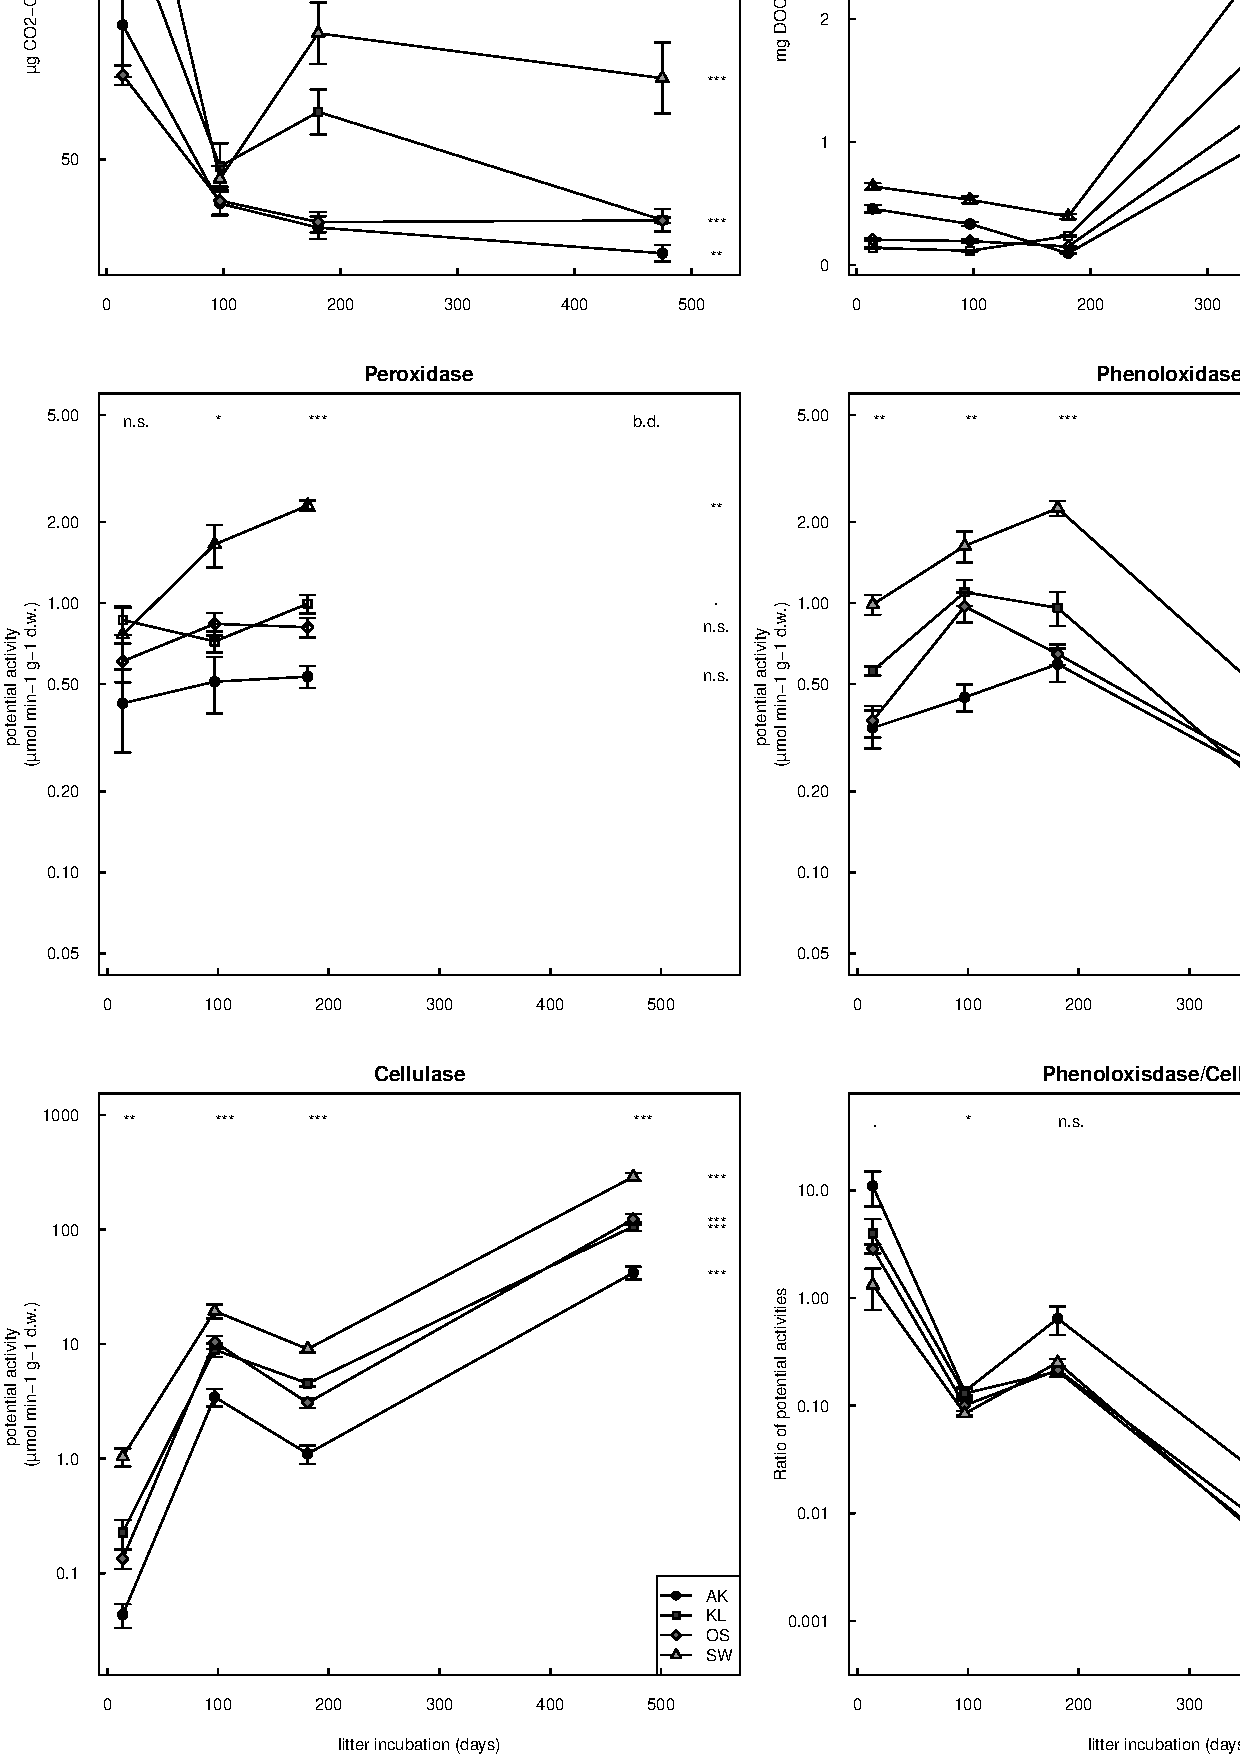
\includegraphics{ligpaper-enz}
\end{center}
\caption{
{\bf Respiration rates, concentration of soluble organic C and potential extracellular enzyme activities} in decomposing beech leaf litter from a mesocosm experiment. Beech litter was collected in: triangles, Schottenwald (SW); diamonds, Ossiach (OS); squares, Klaus-nleopoldsdorf (KL); circles, Achenkirch, AK. Error bars indicate standard errors (n=5). Significant differences between litter types are presented by asterisks above the symbols, significant differences between time points by asterisks to the right of the curves. *, P\textless 0.05, **, P\textless 0.01, ***, P\textless 0.001, b.d. - below detection limit.}
\label{fig:enz}
\end{figure}

\begin{figure}[!ht]
\begin{center}
%\setkeys{Gin}{width=4in}
\setkeys{Gin}{width=\textwidth}
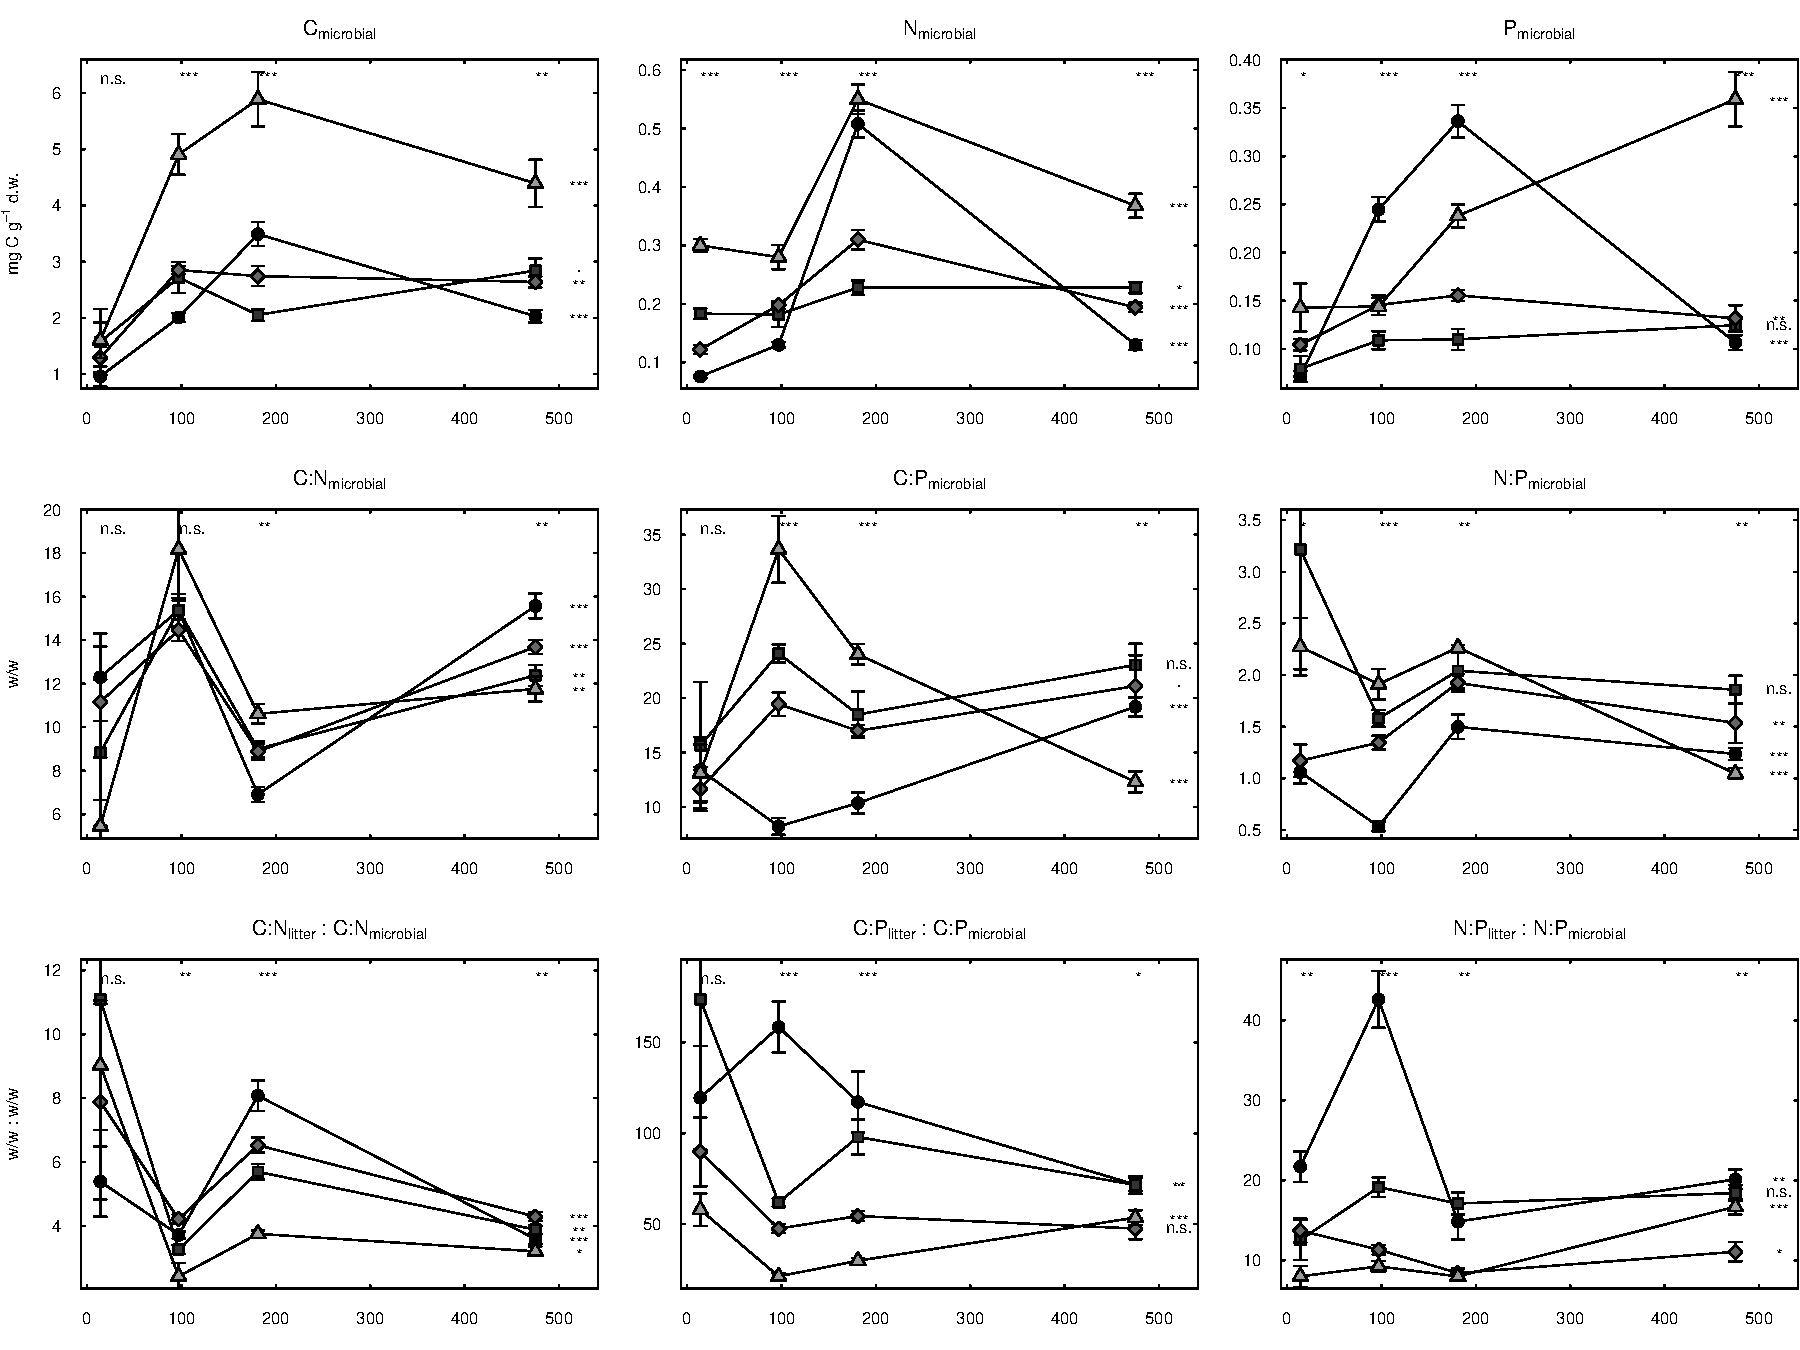
\includegraphics{ligpaper-mb}
\end{center}
\caption{
{\bf Microbial biomass C, N and P, microbial C:N:P stoichiometry and resource/consumer stoichiometric imbalance in these elements}in decomposing beech leaf litter from a mesocosm experiment. Beech litter was collected in: triangles, Schottenwald (SW); diamonds, Ossiach (OS); squares, Klausenleopoldsdorf (KL); circles, Achenkirch, AK. Error bars indicate standard errors (n=5). Significant differences between litter types are presented by asterisks above the symbols, significant differences between time points by asterisks to the right of the curves. *, P\textless 0.05, **, P\textless 0.01, ***, P\textless 0.001.}
\label{fig:mb}
\end{figure}

\begin{figure}[!ht]
\begin{center}
\setkeys{Gin}{width=0.7\textwidth}
%\inputgraphics[width=4in]{figure_name.2.eps}
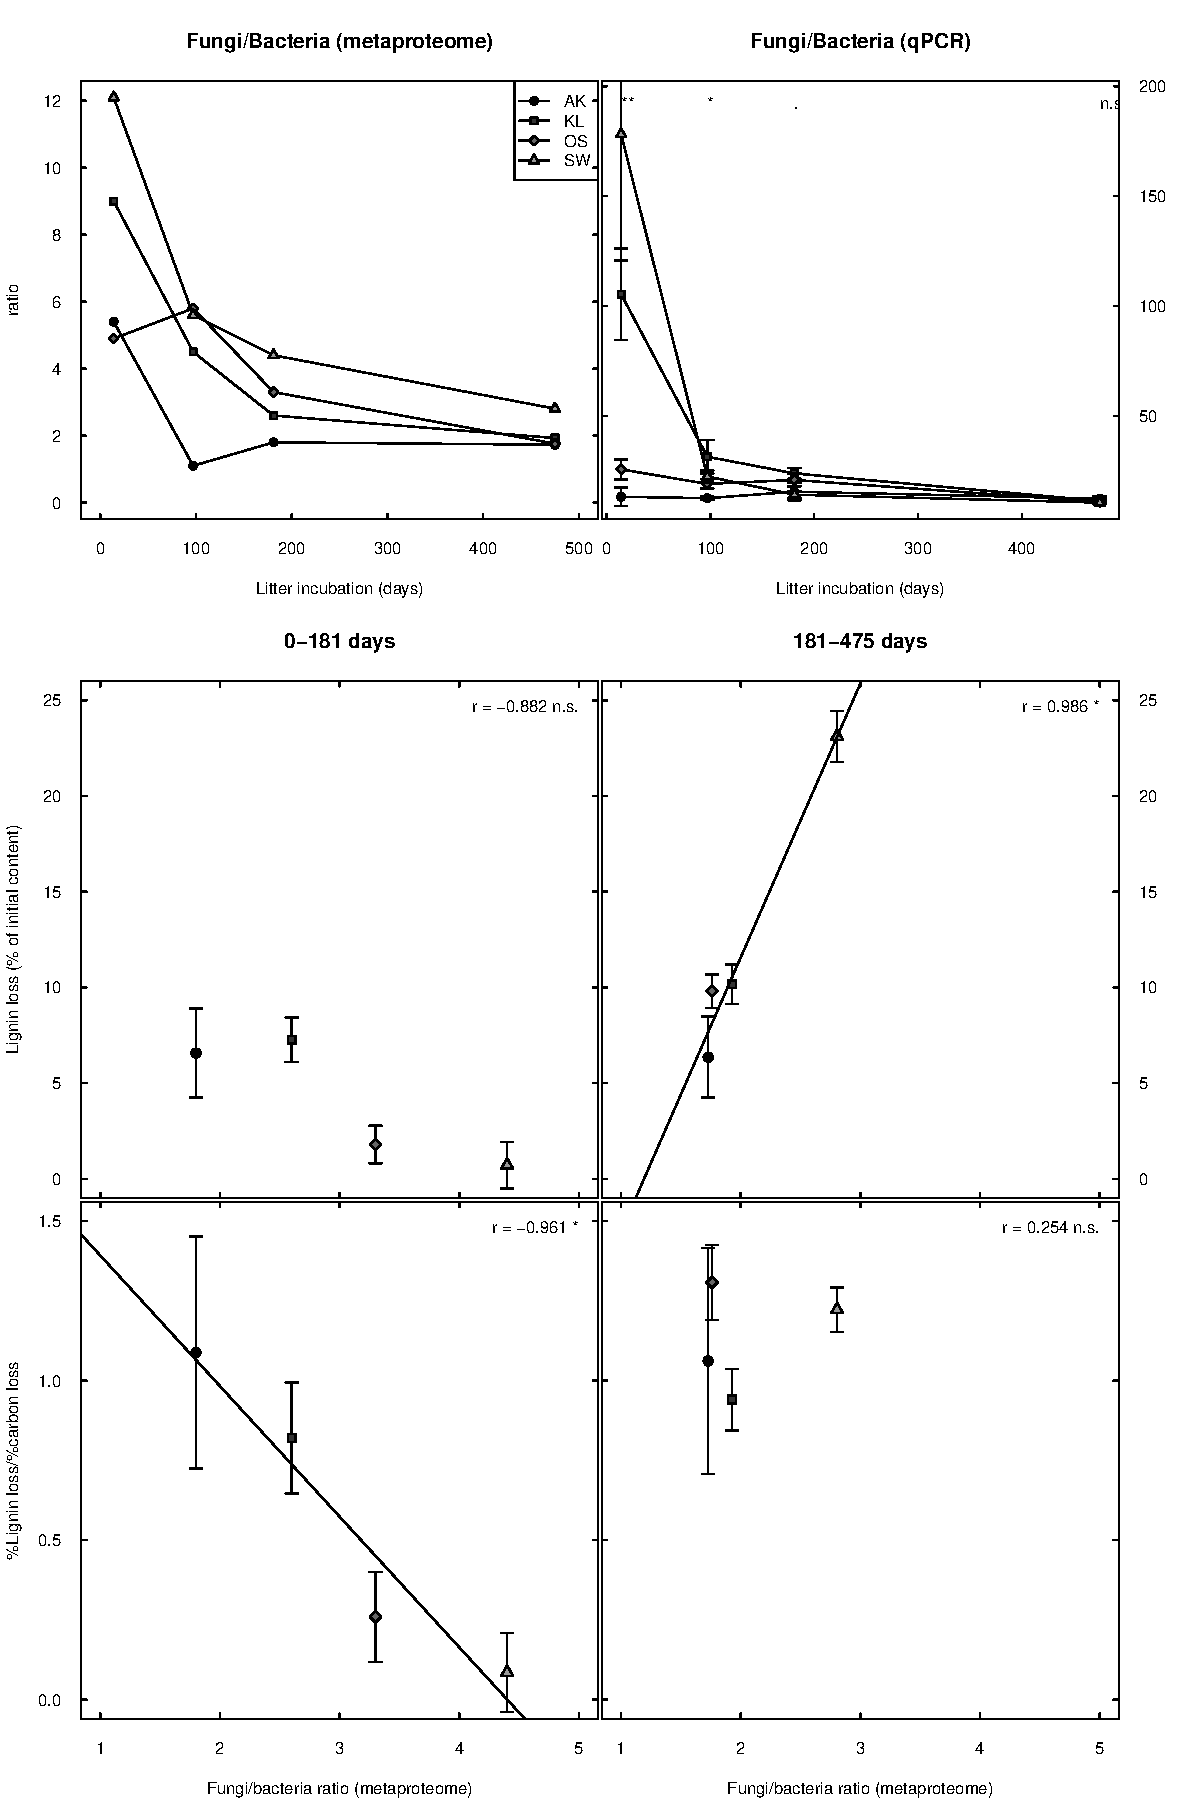
\includegraphics{ligpaper-f2bnew}
\end{center}
\caption{
{\bf Fungi:Bacteria (F:B) ratios and their correlations with LCI change:} Top: F:B protein abundance (left) and DNA (right) ratio. Bottom: Correlations between F:B preotein abundance ratios and Lignin loss (mid) and lignin loss / carbon loss (bottom) for 0-6 months (left) and 6-15 months (right..Errorbars indicate standard errors (n=4-5).  Beech litter was collected in: triangles, Schottenwald (SW); diamonds, Ossiach (OS); squares, Klausenleopoldsdorf (KL); circles, Achenkirch, AK. Error bars indicate standard errors (n=5). Significant differences between litter types are presented by asterisks above the symbols, significant differences between time points by asterisks to the right of the curves. *, P\textless 0.05, **, P\textless 0.01, ***, P\textless 0.001.}
\label{fig:f2b}
\end{figure}

\newpage
\begin{figure}[!ht]
\begin{center}
%\setkeys{Gin}{width=4in}
\setkeys{Gin}{width=\textwidth}
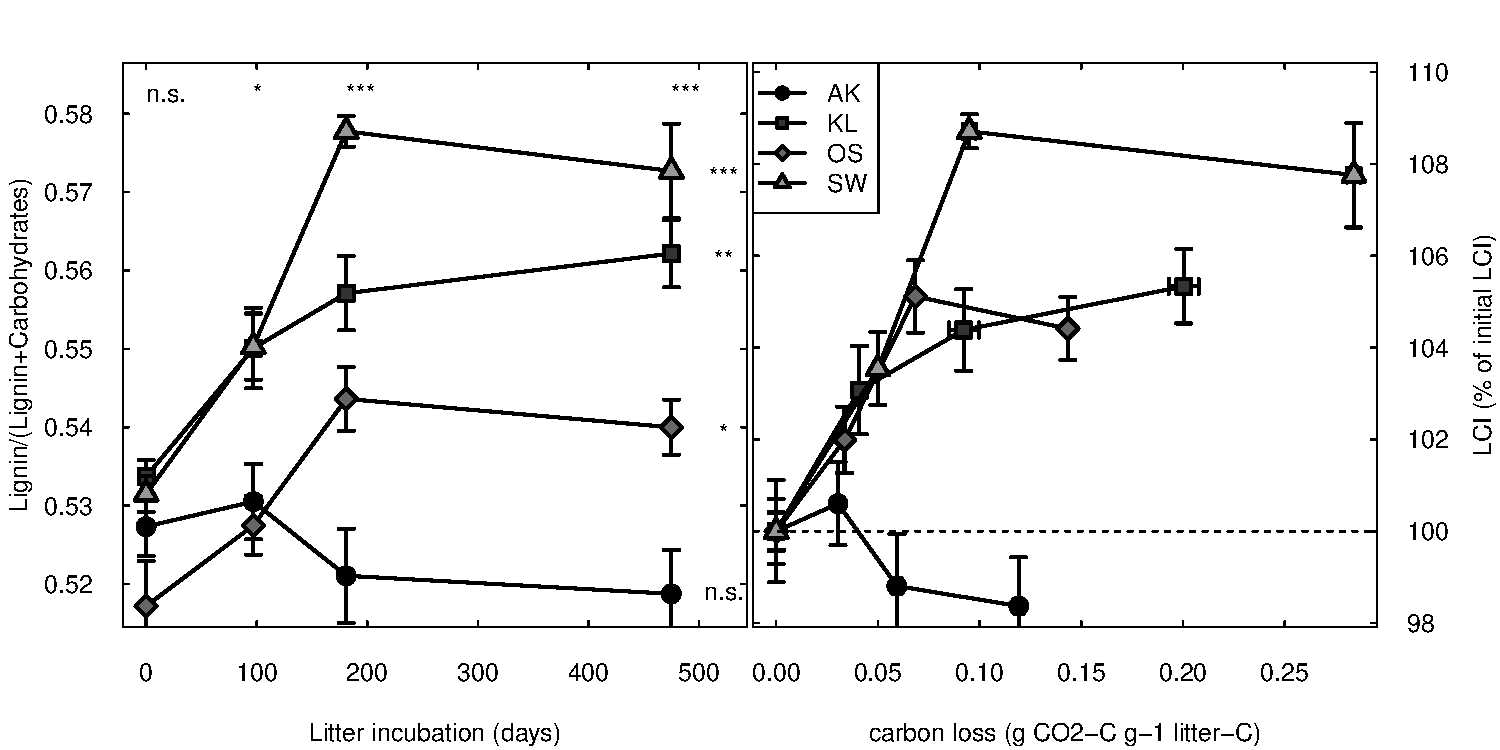
\includegraphics{ligpaper-lci}
\end{center}
\caption{
{\bf Develoment of the LCI (lignin/(lignin+carbohydrates))} during time of beech litter decomposition (A) or plotted against cumulative C loss (B). Errorbars indicate standard errors (n=4-5). The dashed line indicates a constant ratio between lignin and carbohydrates (i.e. no preferential decomposition of carbohydrates. Beech litter was collected in: triangles, Schottenwald (SW); diamonds, Ossiach (OS); squares, Klausenleopoldsdorf (KL); circles, Achenkirch, AK. Error bars indicate standard errors (n=5). Significant differences between litter types are presented by asterisks above the symbols, significant differences between time points by asterisks to the right of the curves. *, P\textless 0.05, **, P\textless 0.01, ***, P\textless 0.001.}
\label{fig:lci}
\end{figure}


\newpage
\begin{figure*}[h!]
\vspace*{2mm}
\begin{center}
\setkeys{Gin}{width=\textwidth}
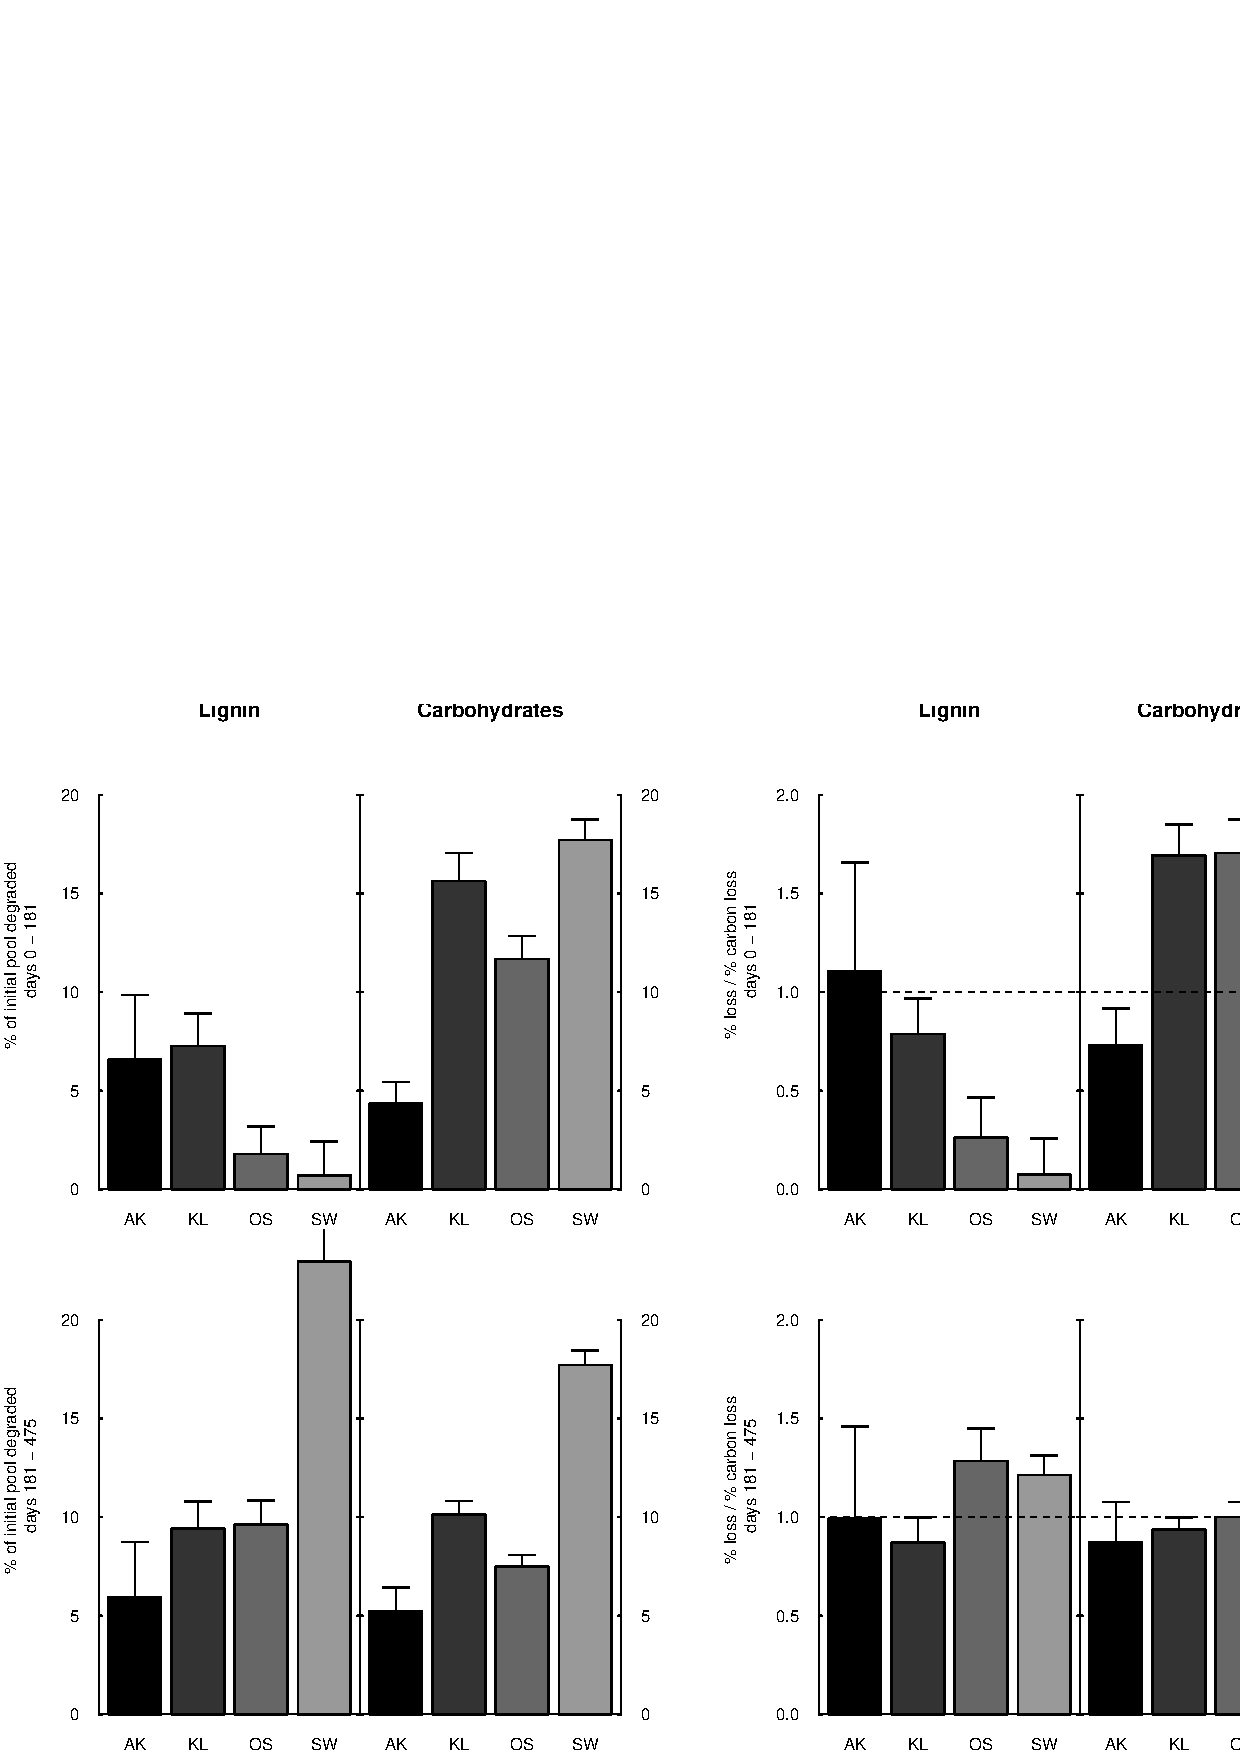
\includegraphics{ligpaper-degrdiff}
\end{center}
\caption{
{\bf Carbon loss corrected amounts of lignin and carbohydrates} degraded in beech litter collected in Achenkirch (AK), Klausenleopoldsdorf (KL), Ossiach (OS) and Schottenwald (SW). Carbon loss was calculated based on accumulated respiration for each mesocosm. Error bars indicate standard errors (n=4-5). The dashed line marks no discrimation during decomposition between lignin, carbohydrates and bulk carbon}
\label{fig:degr}
\end{figure*}

\newpage
\begin{figure*}[h!]
\vspace*{2mm}
\begin{center}
\setkeys{Gin}{width=\textwidth}
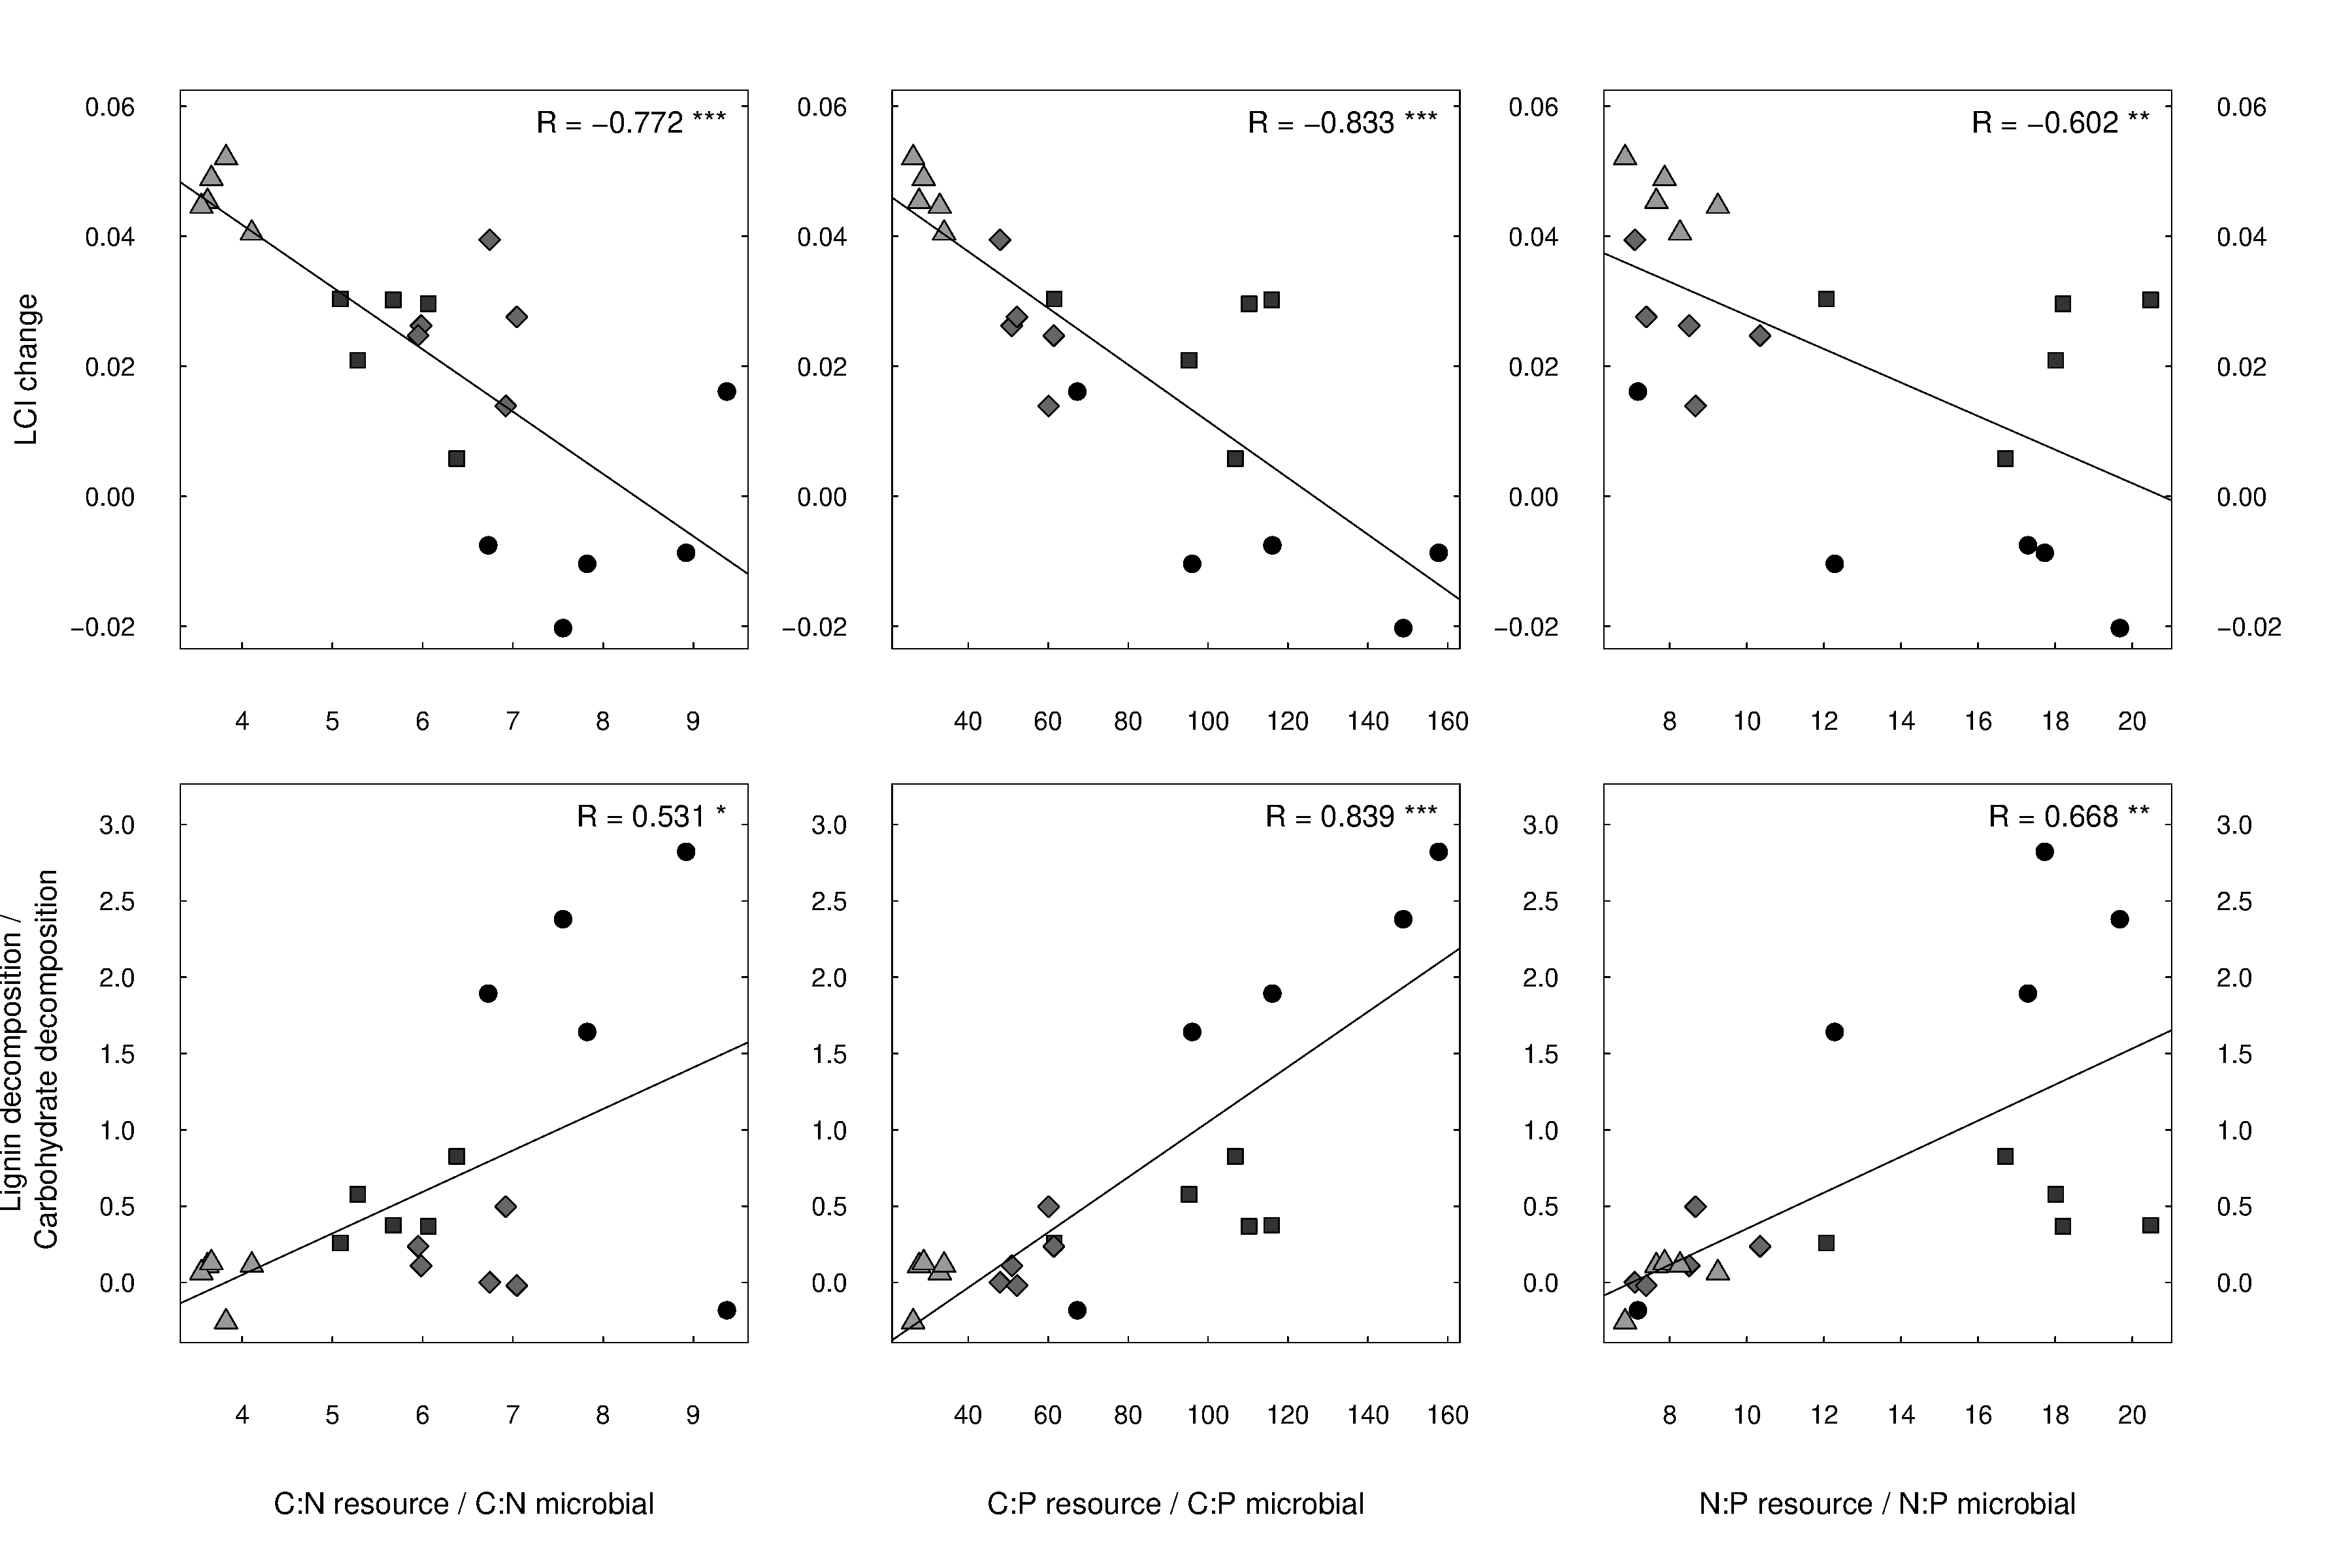
\includegraphics{ligpaper-graphcorr}
\end{center}
\caption{
{\bf Correlation between the LCI change or the ratio of lignin/carbohydrate decomposition ratio during the first 6 months of litter decomposition correlate to litter/microbe stoichiometric imbalances.} and change and Correlations between lignin accumulation during the first 6 month of litter incubation and stoichiometric resource:consumer imbalances. LCI is calculates as of lignin/(lignin+Carbohydrates).  Beech litter was collected in: triangles, Schottenwald (SW); diamonds, Ossiach (OS); squares, Klausenleopoldsdorf (KL); circles, Achenkirch, AK. *, P\textless 0.05, **, P\textless 0.01, ***, P\textless 0.001.}
\label{fig:cor1}
\end{figure*}


\newpage
\begin{figure*}[h!]
\vspace*{2mm}
\begin{center}
\setkeys{Gin}{width=\textwidth}
\begin{Schunk}
\begin{Sinput}
> plot.meta <- function(ord, arrows = F, envfit = T, enz = F, spe.mult = 1, 
+     site.mult = 1, lab = "PCA", choices = 1:2, ...) {
+     choices <- 1:2
+     xvar <- eigenvals(ord)/sum(eigenvals(ord))
+     plot(ord, choices = choices, type = "n", tck = 0.01, xlab = paste(lab, 
+         choices[1], formatC(xvar[choices[1]] * 100, digits = 3), 
+         "% variance"), ylab = paste(lab, choices[2], formatC(xvar[choices[2]] * 
+         100, digits = 3), "% variance"))
+     points(scores(ord, display = "sites", choices = choices) * 
+         site.mult, pch = pch.met, bg = col.met, cex = 1)
+     text(scores(ord, display = "species", choices = choices) * 
+         spe.mult, labels = labels.metaprot, cex = 0.5)
+     if (arrows == T) {
+         arrows(rep(0, length(scores(ord, display = "bp", choices = choices))), 
+             rep(0, length(scores(ord, display = "bp"))), scores(ord, 
+                 display = "bp", choices = choices[1]) * 2, scores(ord, 
+                 display = "bp", choices = choices[2]) * 2, length = 0.1, 
+             angle = 10)
+         text(scores(ord, display = "bp", choices = choices) * 
+             2.4, labels = rownames(scores(ord, display = "bp", 
+             choices = choices)), cex = 0.5)
+     }
+     lims <- par("usr")
+     xspa <- (lims[2] - lims[1])/50
+     yspa <- (lims[4] - lims[3])/50
+     xmin <- tapply(scores(ord, display = "sites", choices = choices[1]), 
+         metaprot.red$Harvest, min)
+     xmax <- tapply(scores(ord, display = "sites", choices = choices[1]), 
+         metaprot.red$Harvest, max)
+     ymin <- tapply(scores(ord, display = "sites", choices = choices[2]), 
+         metaprot.red$Harvest, min)
+     ymax <- tapply(scores(ord, display = "sites", choices = choices[2]), 
+         metaprot.red$Harvest, max)
+     for (i in 1:4) rect(xmin[i] * site.mult - xspa, ymin[i] * 
+         site.mult - yspa, xmax[i] * site.mult + xspa, ymax[i] * 
+         site.mult + yspa)
+     if (envfit == T) {
+         fit.var <- data.frame(alldata$days[cond])
+         colnames(fit.var) <- "Incubation time"
+         plot(envfit(ord, fit.var, choices = choices), cex = 0.5, 
+             p.max = 0.05)
+         fit.var2 <- alldata[cond, 38:43]
+         colnames(fit.var2) <- c("C lit", "N lit", "P lit", "C:N lit", 
+             "C:P lit", "N:P lit")
+         plot(envfit(ord, fit.var2, choices = choices), cex = 0.5, 
+             p.max = 0.05)
+         fit.var3 <- alldata[cond, 50:55]
+         colnames(fit.var3) <- c("C mic", "N mic", "P mic", "C:N mic", 
+             "C:P mic", "N:P mic")
+         plot(envfit(ord, fit.var3, choices = choices), cex = 0.5, 
+             p.max = 0.05)
+         fit.var4 <- alldata[cond, 75:77]
+         colnames(fit.var4) <- c("C:N imb", "C:P imb", "N:P imb")
+         plot(envfit(ord, fit.var4, choices = choices), cex = 0.5, 
+             p.max = 0.05)
+         fit.var5 <- data.frame(metaprot.red[, 4])
+         colnames(fit.var5) <- "F:B"
+         plot(envfit(ord, fit.var5, choices = choices), cex = 0.5, 
+             p.max = 0.05)
+     }
+     if (enz == T) {
+         fit.enz <- data.frame(alldata$phen2cell[cond], alldata[cond, 
+             11:16]/alldata$C_mic[cond])
+         colnames(fit.enz) <- c("Phen:Cell", "Cell", "Chit", "Phos", 
+             "Prot", "Pero", "Phen")
+         plot(envfit(ord, fit.enz, choices = choices), cex = 0.5, 
+             p.max = 0.05)
+     }
+ }
> require("fields")
> metaprot.red <- metaprot[which(is.na(metaprot[6]) == F), T]
> metaprot.red[6:ncol(metaprot.red)] <- metaprot.red[6:ncol(metaprot.red)]/rowSums(metaprot.red[6:ncol(metaprot.red)])
> pch.met <- c(21, 21, 21, 21, 22, 22, 22, 22, 23, 23, 23, 23, 
+     24, 24, 24, 24)
> col.met <- c("#000000", "#333333", "#666666", "#999999", "#000000", 
+     "#333333", "#666666", "#999999", "#000000", "#333333", "#666666", 
+     "#999999", "#000000", "#333333", "#666666", "#999999")
> labels.metaprot <- c("Doth", "Euro", "Leot", "Sacc", "Sord", 
+     "Agar", "Trem", "Usti", "Ther", "Bact", "Acti", "Cyan", "Firm", 
+     "Fuso", "Verr", "Dict", "Alph", "Beta", "Gamm", "Delt", "Epsi")
> cond <- which(is.na(metaprot[6]) == F)
> ord <- cca(metaprot.red[6:ncol(metaprot.red)])
> plot.meta(ord, arrows = T, envfit = T, enz = F)